\documentclass[1p]{elsarticle_modified}
%\bibliographystyle{elsarticle-num}

%\usepackage[colorlinks]{hyperref}
%\usepackage{abbrmath_seonhwa} %\Abb, \Ascr, \Acal ,\Abf, \Afrak
\usepackage{amsfonts}
\usepackage{amssymb}
\usepackage{amsmath}
\usepackage{amsthm}
\usepackage{scalefnt}
\usepackage{amsbsy}
\usepackage{kotex}
\usepackage{caption}
\usepackage{subfig}
\usepackage{color}
\usepackage{graphicx}
\usepackage{xcolor} %% white, black, red, green, blue, cyan, magenta, yellow
\usepackage{float}
\usepackage{setspace}
\usepackage{hyperref}

\usepackage{tikz}
\usetikzlibrary{arrows}

\usepackage{multirow}
\usepackage{array} % fixed length table
\usepackage{hhline}

%%%%%%%%%%%%%%%%%%%%%
\makeatletter
\renewcommand*\env@matrix[1][\arraystretch]{%
	\edef\arraystretch{#1}%
	\hskip -\arraycolsep
	\let\@ifnextchar\new@ifnextchar
	\array{*\c@MaxMatrixCols c}}
\makeatother %https://tex.stackexchange.com/questions/14071/how-can-i-increase-the-line-spacing-in-a-matrix
%%%%%%%%%%%%%%%

\usepackage[normalem]{ulem}

\newcommand{\msout}[1]{\ifmmode\text{\sout{\ensuremath{#1}}}\else\sout{#1}\fi}
%SOURCE: \msout is \stkout macro in https://tex.stackexchange.com/questions/20609/strikeout-in-math-mode

\newcommand{\cancel}[1]{
	\ifmmode
	{\color{red}\msout{#1}}
	\else
	{\color{red}\sout{#1}}
	\fi
}

\newcommand{\add}[1]{
	{\color{blue}\uwave{#1}}
}

\newcommand{\replace}[2]{
	\ifmmode
	{\color{red}\msout{#1}}{\color{blue}\uwave{#2}}
	\else
	{\color{red}\sout{#1}}{\color{blue}\uwave{#2}}
	\fi
}

\newcommand{\Sol}{\mathcal{S}} %segment
\newcommand{\D}{D} %diagram
\newcommand{\A}{\mathcal{A}} %arc


%%%%%%%%%%%%%%%%%%%%%%%%%%%%%5 test

\def\sl{\operatorname{\textup{SL}}(2,\Cbb)}
\def\psl{\operatorname{\textup{PSL}}(2,\Cbb)}
\def\quan{\mkern 1mu \triangleright \mkern 1mu}

\theoremstyle{definition}
\newtheorem{thm}{Theorem}[section]
\newtheorem{prop}[thm]{Proposition}
\newtheorem{lem}[thm]{Lemma}
\newtheorem{ques}[thm]{Question}
\newtheorem{cor}[thm]{Corollary}
\newtheorem{defn}[thm]{Definition}
\newtheorem{exam}[thm]{Example}
\newtheorem{rmk}[thm]{Remark}
\newtheorem{alg}[thm]{Algorithm}

\newcommand{\I}{\sqrt{-1}}
\begin{document}

%\begin{frontmatter}
%
%\title{Boundary parabolic representations of knots up to 8 crossings}
%
%%% Group authors per affiliation:
%\author{Yunhi Cho} 
%\address{Department of Mathematics, University of Seoul, Seoul, Korea}
%\ead{yhcho@uos.ac.kr}
%
%
%\author{Seonhwa Kim} %\fnref{s_kim}}
%\address{Center for Geometry and Physics, Institute for Basic Science, Pohang, 37673, Korea}
%\ead{ryeona17@ibs.re.kr}
%
%\author{Hyuk Kim}
%\address{Department of Mathematical Sciences, Seoul National University, Seoul 08826, Korea}
%\ead{hyukkim@snu.ac.kr}
%
%\author{Seokbeom Yoon}
%\address{Department of Mathematical Sciences, Seoul National University, Seoul, 08826,  Korea}
%\ead{sbyoon15@snu.ac.kr}
%
%\begin{abstract}
%We find all boundary parabolic representation of knots up to 8 crossings.
%
%\end{abstract}
%\begin{keyword}
%    \MSC[2010] 57M25 
%\end{keyword}
%
%\end{frontmatter}

%\linenumbers
%\tableofcontents
%
\newcommand\colored[1]{\textcolor{white}{\rule[-0.35ex]{0.8em}{1.4ex}}\kern-0.8em\color{red} #1}%
%\newcommand\colored[1]{\textcolor{white}{ #1}\kern-2.17ex	\textcolor{white}{ #1}\kern-1.81ex	\textcolor{white}{ #1}\kern-2.15ex\color{red}#1	}

{\Large $\underline{11a_{28}~(K11a_{28})}$}

\setlength{\tabcolsep}{10pt}
\renewcommand{\arraystretch}{1.6}
\vspace{1cm}\begin{tabular}{m{100pt}>{\centering\arraybackslash}m{274pt}}
\multirow{5}{120pt}{
	\centering
	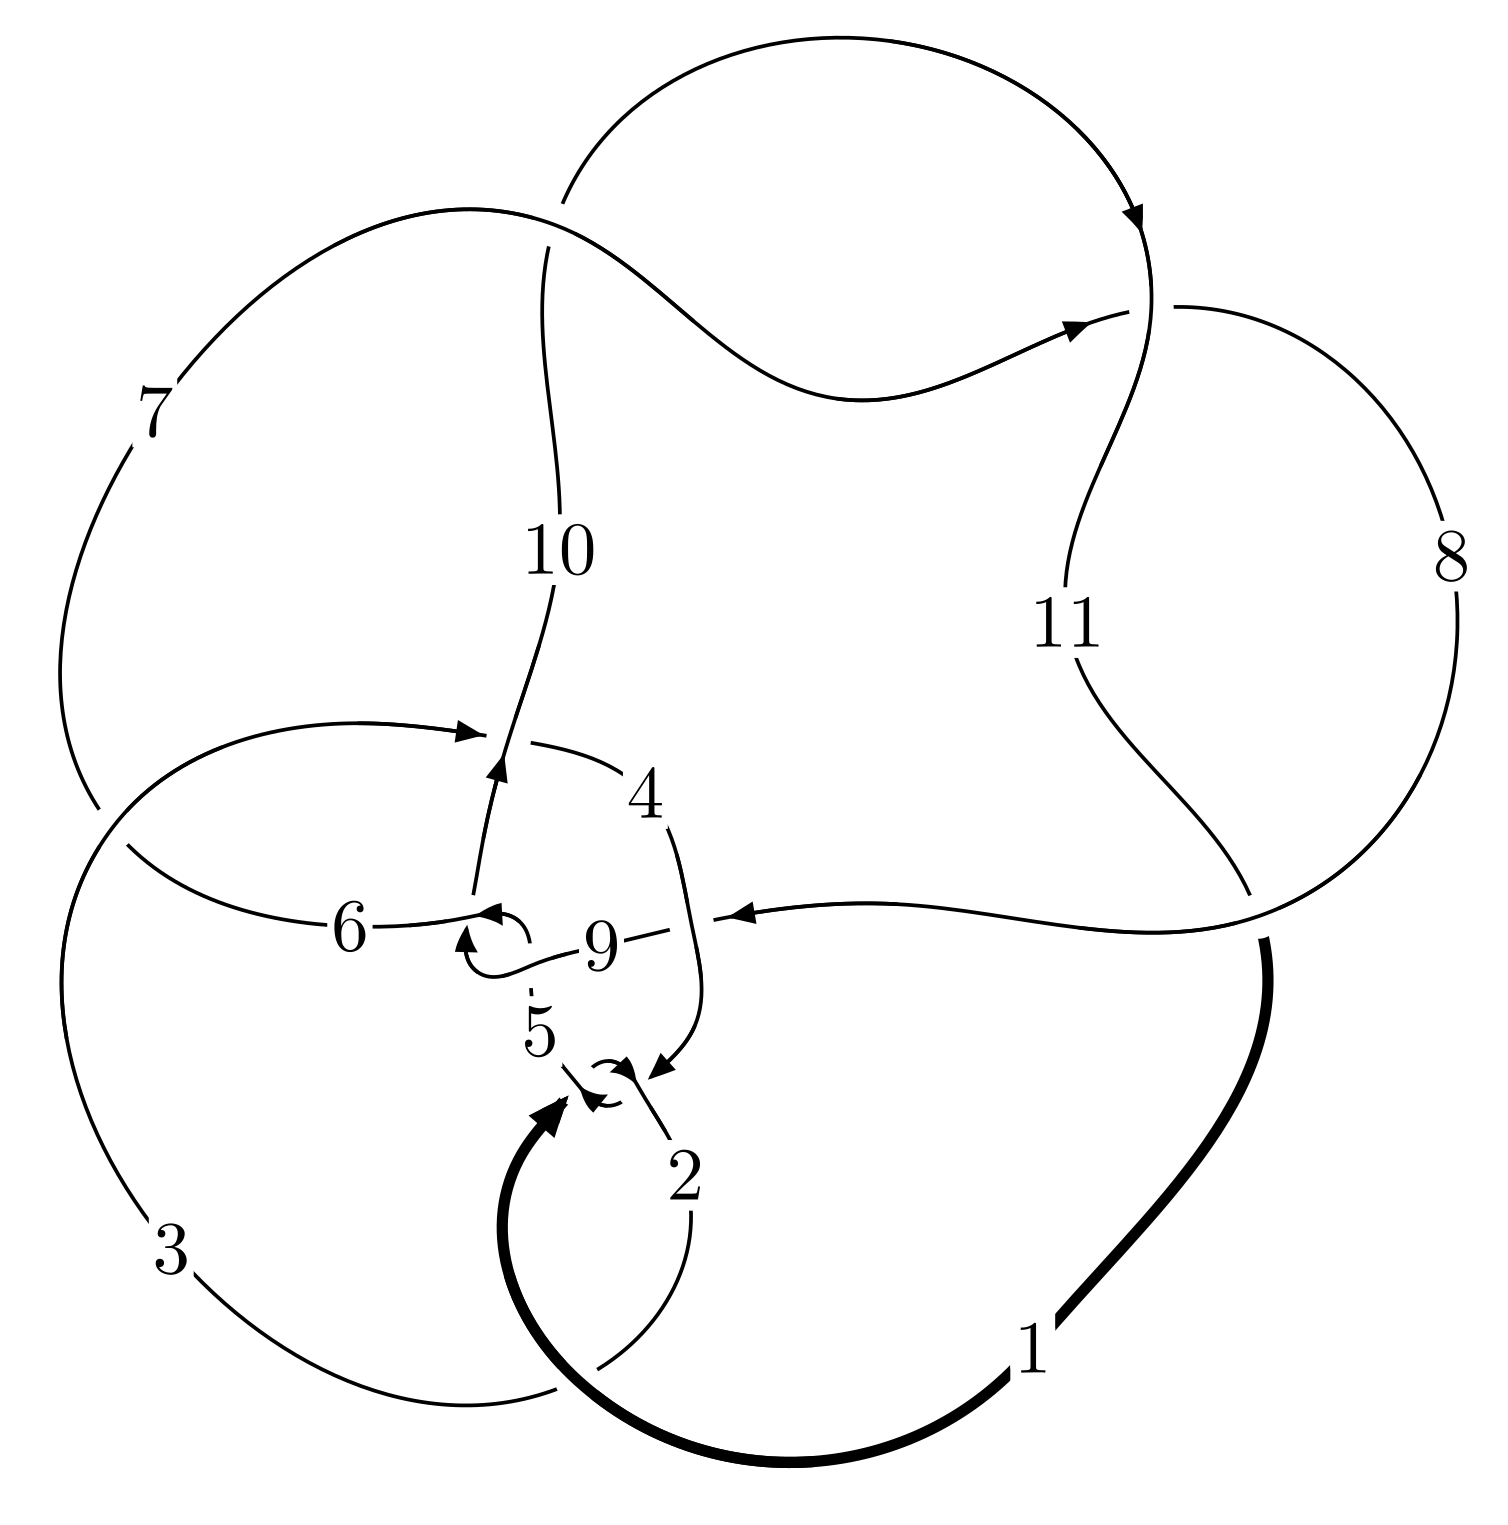
\includegraphics[width=112pt]{../../../GIT/diagram.site/Diagrams/png/277_11a_28.png}\\
\ \ \ A knot diagram\footnotemark}&
\allowdisplaybreaks
\textbf{Linearized knot diagam} \\
\cline{2-2}
 &
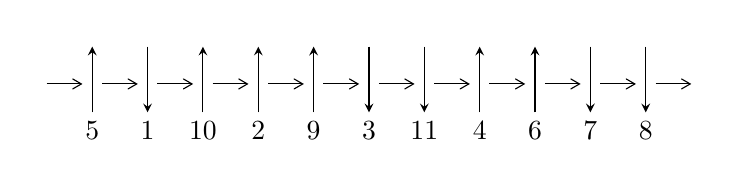
\begin{tikzpicture}[x=20pt, y=17pt]
	% nodes
	\node (C0) at (0, 0) {};
	\node (C1) at (1, 0) {};
	\node (C1U) at (1, +1) {};
	\node (C1D) at (1, -1) {5};

	\node (C2) at (2, 0) {};
	\node (C2U) at (2, +1) {};
	\node (C2D) at (2, -1) {1};

	\node (C3) at (3, 0) {};
	\node (C3U) at (3, +1) {};
	\node (C3D) at (3, -1) {10};

	\node (C4) at (4, 0) {};
	\node (C4U) at (4, +1) {};
	\node (C4D) at (4, -1) {2};

	\node (C5) at (5, 0) {};
	\node (C5U) at (5, +1) {};
	\node (C5D) at (5, -1) {9};

	\node (C6) at (6, 0) {};
	\node (C6U) at (6, +1) {};
	\node (C6D) at (6, -1) {3};

	\node (C7) at (7, 0) {};
	\node (C7U) at (7, +1) {};
	\node (C7D) at (7, -1) {11};

	\node (C8) at (8, 0) {};
	\node (C8U) at (8, +1) {};
	\node (C8D) at (8, -1) {4};

	\node (C9) at (9, 0) {};
	\node (C9U) at (9, +1) {};
	\node (C9D) at (9, -1) {6};

	\node (C10) at (10, 0) {};
	\node (C10U) at (10, +1) {};
	\node (C10D) at (10, -1) {7};

	\node (C11) at (11, 0) {};
	\node (C11U) at (11, +1) {};
	\node (C11D) at (11, -1) {8};
	\node (C12) at (12, 0) {};

	% arrows
	\draw[->,>={angle 60}]
	(C0) edge (C1) (C1) edge (C2) (C2) edge (C3) (C3) edge (C4) (C4) edge (C5) (C5) edge (C6) (C6) edge (C7) (C7) edge (C8) (C8) edge (C9) (C9) edge (C10) (C10) edge (C11) (C11) edge (C12) ;	\draw[->,>=stealth]
	(C1D) edge (C1U) (C2U) edge (C2D) (C3D) edge (C3U) (C4D) edge (C4U) (C5D) edge (C5U) (C6U) edge (C6D) (C7U) edge (C7D) (C8D) edge (C8U) (C9D) edge (C9U) (C10U) edge (C10D) (C11U) edge (C11D) ;
	\end{tikzpicture} \\
\hhline{~~} \\& 
\textbf{Solving Sequence} \\ \cline{2-2} 
 &
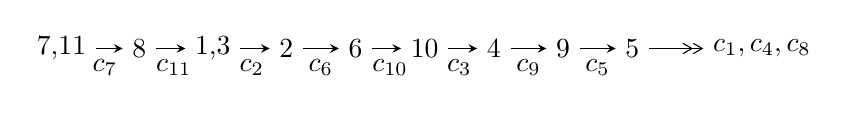
\begin{tikzpicture}[x=25pt, y=7pt]
	% node
	\node (A0) at (-1/8, 0) {7,11};
	\node (A1) at (1, 0) {8};
	\node (A2) at (33/16, 0) {1,3};
	\node (A3) at (25/8, 0) {2};
	\node (A4) at (33/8, 0) {6};
	\node (A5) at (41/8, 0) {10};
	\node (A6) at (49/8, 0) {4};
	\node (A7) at (57/8, 0) {9};
	\node (A8) at (65/8, 0) {5};
	\node (C1) at (1/2, -1) {$c_{7}$};
	\node (C2) at (3/2, -1) {$c_{11}$};
	\node (C3) at (21/8, -1) {$c_{2}$};
	\node (C4) at (29/8, -1) {$c_{6}$};
	\node (C5) at (37/8, -1) {$c_{10}$};
	\node (C6) at (45/8, -1) {$c_{3}$};
	\node (C7) at (53/8, -1) {$c_{9}$};
	\node (C8) at (61/8, -1) {$c_{5}$};
	\node (A9) at (10, 0) {$c_{1},c_{4},c_{8}$};

	% edge
	\draw[->,>=stealth]	
	(A0) edge (A1) (A1) edge (A2) (A2) edge (A3) (A3) edge (A4) (A4) edge (A5) (A5) edge (A6) (A6) edge (A7) (A7) edge (A8) ;
	\draw[->>,>={angle 60}]	
	(A8) edge (A9);
\end{tikzpicture} \\ 

\end{tabular} \\

\footnotetext{
The image of knot diagram is generated by the software ``\textbf{Draw programme}" developed by Andrew Bartholomew(\url{http://www.layer8.co.uk/maths/draw/index.htm\#Running-draw}), where we modified some parts for our purpose(\url{https://github.com/CATsTAILs/LinksPainter}).
}\phantom \\ \newline 
\centering \textbf{Ideals for irreducible components\footnotemark of $X_{\text{par}}$} 
 
\begin{align*}
I^u_{1}&=\langle 
2.01615\times10^{63} u^{59}-7.91768\times10^{63} u^{58}+\cdots+1.22570\times10^{63} b-6.80954\times10^{62},\\
\phantom{I^u_{1}}&\phantom{= \langle  }4.32115\times10^{62} u^{59}-2.12406\times10^{63} u^{58}+\cdots+4.08568\times10^{62} a-3.28832\times10^{62},\;u^{60}-5 u^{59}+\cdots+5 u^2+1\rangle \\
\\
\end{align*}
\raggedright * 1 irreducible components of $\dim_{\mathbb{C}}=0$, with total 60 representations.\\
\footnotetext{All coefficients of polynomials are rational numbers. But the coefficients are sometimes approximated in decimal forms when there is not enough margin.}
\newpage
\renewcommand{\arraystretch}{1}
\centering \section*{I. $I^u_{1}= \langle 2.02\times10^{63} u^{59}-7.92\times10^{63} u^{58}+\cdots+1.23\times10^{63} b-6.81\times10^{62},\;4.32\times10^{62} u^{59}-2.12\times10^{63} u^{58}+\cdots+4.09\times10^{62} a-3.29\times10^{62},\;u^{60}-5 u^{59}+\cdots+5 u^2+1 \rangle$}
\flushleft \textbf{(i) Arc colorings}\\
\begin{tabular}{m{7pt} m{180pt} m{7pt} m{180pt} }
\flushright $a_{7}=$&$\begin{pmatrix}1\\0\end{pmatrix}$ \\
\flushright $a_{11}=$&$\begin{pmatrix}0\\u\end{pmatrix}$ \\
\flushright $a_{8}=$&$\begin{pmatrix}1\\u^2\end{pmatrix}$ \\
\flushright $a_{1}=$&$\begin{pmatrix}- u\\- u^3+u\end{pmatrix}$ \\
\flushright $a_{3}=$&$\begin{pmatrix}-1.05763 u^{59}+5.19879 u^{58}+\cdots-2.64467 u+0.804841\\-1.64489 u^{59}+6.45970 u^{58}+\cdots-0.851795 u+0.555561\end{pmatrix}$ \\
\flushright $a_{2}=$&$\begin{pmatrix}-3.61502 u^{59}+14.3888 u^{58}+\cdots+0.169951 u+2.62747\\-3.69618 u^{59}+14.2840 u^{58}+\cdots-1.10903 u+2.32983\end{pmatrix}$ \\
\flushright $a_{6}=$&$\begin{pmatrix}0.370829 u^{59}-0.610393 u^{58}+\cdots+4.23462 u+0.393300\\-1.17480 u^{59}+5.71906 u^{58}+\cdots+2.79612 u+1.18421\end{pmatrix}$ \\
\flushright $a_{10}=$&$\begin{pmatrix}u\\u\end{pmatrix}$ \\
\flushright $a_{4}=$&$\begin{pmatrix}-2.95589 u^{59}+12.2653 u^{58}+\cdots-2.05741 u+2.48023\\-3.54315 u^{59}+13.5262 u^{58}+\cdots-0.264534 u+2.23095\end{pmatrix}$ \\
\flushright $a_{9}=$&$\begin{pmatrix}3.21953 u^{59}-12.4002 u^{58}+\cdots+0.378631 u-1.25671\\5.61791 u^{59}-21.2160 u^{58}+\cdots+0.447850 u-2.31429\end{pmatrix}$ \\
\flushright $a_{5}=$&$\begin{pmatrix}3.31846 u^{59}-11.7462 u^{58}+\cdots-0.711385 u-2.30380\\3.31846 u^{59}-11.7462 u^{58}+\cdots-2.71138 u-2.30380\end{pmatrix}$\\ \flushright $a_{5}=$&$\begin{pmatrix}3.31846 u^{59}-11.7462 u^{58}+\cdots-0.711385 u-2.30380\\3.31846 u^{59}-11.7462 u^{58}+\cdots-2.71138 u-2.30380\end{pmatrix}$\\&\end{tabular}
\flushleft \textbf{(ii) Obstruction class $= -1$}\\~\\
\flushleft \textbf{(iii) Cusp Shapes $= -10.2583 u^{59}+32.5172 u^{58}+\cdots+12.1083 u+12.4600$}\\~\\
\newpage\renewcommand{\arraystretch}{1}
\flushleft \textbf{(iv) u-Polynomials at the component}\newline \\
\begin{tabular}{m{50pt}|m{274pt}}
Crossings & \hspace{64pt}u-Polynomials at each crossing \\
\hline $$\begin{aligned}c_{1},c_{4}\end{aligned}$$&$\begin{aligned}
&u^{60}+u^{59}+\cdots-2 u+1
\end{aligned}$\\
\hline $$\begin{aligned}c_{2}\end{aligned}$$&$\begin{aligned}
&u^{60}+25 u^{59}+\cdots+6 u+1
\end{aligned}$\\
\hline $$\begin{aligned}c_{3}\end{aligned}$$&$\begin{aligned}
&u^{60}-3 u^{59}+\cdots-4 u+1
\end{aligned}$\\
\hline $$\begin{aligned}c_{5},c_{9}\end{aligned}$$&$\begin{aligned}
&u^{60}- u^{59}+\cdots+5 u^2+1
\end{aligned}$\\
\hline $$\begin{aligned}c_{6}\end{aligned}$$&$\begin{aligned}
&u^{60}-13 u^{59}+\cdots-46 u-1
\end{aligned}$\\
\hline $$\begin{aligned}c_{7},c_{10},c_{11}\end{aligned}$$&$\begin{aligned}
&u^{60}+5 u^{59}+\cdots+5 u^2+1
\end{aligned}$\\
\hline $$\begin{aligned}c_{8}\end{aligned}$$&$\begin{aligned}
&u^{60}+17 u^{59}+\cdots+288 u+79
\end{aligned}$\\
\hline
\end{tabular}\\~\\
\newpage\renewcommand{\arraystretch}{1}
\flushleft \textbf{(v) Riley Polynomials at the component}\newline \\
\begin{tabular}{m{50pt}|m{274pt}}
Crossings & \hspace{64pt}Riley Polynomials at each crossing \\
\hline $$\begin{aligned}c_{1},c_{4}\end{aligned}$$&$\begin{aligned}
&y^{60}+25 y^{59}+\cdots+6 y+1
\end{aligned}$\\
\hline $$\begin{aligned}c_{2}\end{aligned}$$&$\begin{aligned}
&y^{60}+21 y^{59}+\cdots+62 y+1
\end{aligned}$\\
\hline $$\begin{aligned}c_{3}\end{aligned}$$&$\begin{aligned}
&y^{60}+5 y^{59}+\cdots+30 y+1
\end{aligned}$\\
\hline $$\begin{aligned}c_{5},c_{9}\end{aligned}$$&$\begin{aligned}
&y^{60}-43 y^{59}+\cdots+10 y+1
\end{aligned}$\\
\hline $$\begin{aligned}c_{6}\end{aligned}$$&$\begin{aligned}
&y^{60}+109 y^{59}+\cdots-2526 y+1
\end{aligned}$\\
\hline $$\begin{aligned}c_{7},c_{10},c_{11}\end{aligned}$$&$\begin{aligned}
&y^{60}-59 y^{59}+\cdots+10 y+1
\end{aligned}$\\
\hline $$\begin{aligned}c_{8}\end{aligned}$$&$\begin{aligned}
&y^{60}+73 y^{59}+\cdots-15478 y+6241
\end{aligned}$\\
\hline
\end{tabular}\\~\\
\newpage\flushleft \textbf{(vi) Complex Volumes and Cusp Shapes}
$$\begin{array}{c|c|c}  
\text{Solutions to }I^u_{1}& \I (\text{vol} + \sqrt{-1}CS) & \text{Cusp shape}\\
 \hline 
\begin{aligned}
u &= -0.533782 + 0.834528 I \\
a &= -0.670577 - 0.244749 I \\
b &= -0.90360 + 1.11851 I\end{aligned}
 & \phantom{-}3.66250 + 11.73970 I & \phantom{-0.000000 } 0. - 9.07508 I \\ \hline\begin{aligned}
u &= -0.533782 - 0.834528 I \\
a &= -0.670577 + 0.244749 I \\
b &= -0.90360 - 1.11851 I\end{aligned}
 & \phantom{-}3.66250 - 11.73970 I & \phantom{-0.000000 -}0. + 9.07508 I \\ \hline\begin{aligned}
u &= \phantom{-}0.911823 + 0.442516 I \\
a &= \phantom{-}0.720916 - 0.600914 I \\
b &= \phantom{-}0.661282 + 0.144344 I\end{aligned}
 & -2.94476 - 0.12365 I & \phantom{-0.000000 } 0 \\ \hline\begin{aligned}
u &= \phantom{-}0.911823 - 0.442516 I \\
a &= \phantom{-}0.720916 + 0.600914 I \\
b &= \phantom{-}0.661282 - 0.144344 I\end{aligned}
 & -2.94476 + 0.12365 I & \phantom{-0.000000 } 0 \\ \hline\begin{aligned}
u &= -0.698160 + 0.696499 I \\
a &= -0.527979 + 0.494269 I \\
b &= \phantom{-}0.451910 + 0.688864 I\end{aligned}
 & \phantom{-}4.58804 - 1.10123 I & \phantom{-0.000000 } 0 \\ \hline\begin{aligned}
u &= -0.698160 - 0.696499 I \\
a &= -0.527979 - 0.494269 I \\
b &= \phantom{-}0.451910 - 0.688864 I\end{aligned}
 & \phantom{-}4.58804 + 1.10123 I & \phantom{-0.000000 } 0 \\ \hline\begin{aligned}
u &= \phantom{-}0.481557 + 0.943096 I \\
a &= \phantom{-}0.369140 - 0.171842 I \\
b &= \phantom{-}0.746469 + 0.482040 I\end{aligned}
 & -1.19130 - 5.66306 I & \phantom{-0.000000 } 0 \\ \hline\begin{aligned}
u &= \phantom{-}0.481557 - 0.943096 I \\
a &= \phantom{-}0.369140 + 0.171842 I \\
b &= \phantom{-}0.746469 - 0.482040 I\end{aligned}
 & -1.19130 + 5.66306 I & \phantom{-0.000000 } 0 \\ \hline\begin{aligned}
u &= -0.617210 + 0.869107 I \\
a &= \phantom{-}0.378949 - 0.544669 I \\
b &= -0.494270 - 0.791701 I\end{aligned}
 & \phantom{-}3.47399 - 6.14744 I & \phantom{-0.000000 } 0 \\ \hline\begin{aligned}
u &= -0.617210 - 0.869107 I \\
a &= \phantom{-}0.378949 + 0.544669 I \\
b &= -0.494270 + 0.791701 I\end{aligned}
 & \phantom{-}3.47399 + 6.14744 I & \phantom{-0.000000 } 0\\
 \hline 
 \end{array}$$\newpage$$\begin{array}{c|c|c}  
\text{Solutions to }I^u_{1}& \I (\text{vol} + \sqrt{-1}CS) & \text{Cusp shape}\\
 \hline 
\begin{aligned}
u &= -0.435894 + 0.774361 I \\
a &= \phantom{-}0.472416 + 0.478267 I \\
b &= \phantom{-}0.804781 - 1.056000 I\end{aligned}
 & \phantom{-}5.33401 + 6.06206 I & \phantom{-}5.25486 - 4.79805 I \\ \hline\begin{aligned}
u &= -0.435894 - 0.774361 I \\
a &= \phantom{-}0.472416 - 0.478267 I \\
b &= \phantom{-}0.804781 + 1.056000 I\end{aligned}
 & \phantom{-}5.33401 - 6.06206 I & \phantom{-}5.25486 + 4.79805 I \\ \hline\begin{aligned}
u &= \phantom{-}1.201330 + 0.191717 I \\
a &= \phantom{-}1.064620 - 0.375117 I \\
b &= \phantom{-}0.790732 + 0.105612 I\end{aligned}
 & -2.92701 - 0.02185 I & \phantom{-0.000000 } 0 \\ \hline\begin{aligned}
u &= \phantom{-}1.201330 - 0.191717 I \\
a &= \phantom{-}1.064620 + 0.375117 I \\
b &= \phantom{-}0.790732 - 0.105612 I\end{aligned}
 & -2.92701 + 0.02185 I & \phantom{-0.000000 } 0 \\ \hline\begin{aligned}
u &= \phantom{-}0.240498 + 0.711477 I \\
a &= -0.001003 + 0.236197 I \\
b &= -0.565357 - 0.577780 I\end{aligned}
 & \phantom{-}0.18899 - 1.45187 I & \phantom{-}1.34936 + 5.34755 I \\ \hline\begin{aligned}
u &= \phantom{-}0.240498 - 0.711477 I \\
a &= -0.001003 - 0.236197 I \\
b &= -0.565357 + 0.577780 I\end{aligned}
 & \phantom{-}0.18899 + 1.45187 I & \phantom{-}1.34936 - 5.34755 I \\ \hline\begin{aligned}
u &= -1.27084\phantom{ +0.000000I} \\
a &= -1.71198\phantom{ +0.000000I} \\
b &= -0.0201988\phantom{ +0.000000I}\end{aligned}
 & \phantom{-}1.61104\phantom{ +0.000000I} & \phantom{-0.000000 } 0 \\ \hline\begin{aligned}
u &= -0.529233 + 0.441086 I \\
a &= -1.45011 - 1.15685 I \\
b &= -0.949462 + 0.711668 I\end{aligned}
 & -1.15016 + 4.52322 I & -1.58408 - 7.91740 I \\ \hline\begin{aligned}
u &= -0.529233 - 0.441086 I \\
a &= -1.45011 + 1.15685 I \\
b &= -0.949462 - 0.711668 I\end{aligned}
 & -1.15016 - 4.52322 I & -1.58408 + 7.91740 I \\ \hline\begin{aligned}
u &= \phantom{-}1.310500 + 0.080285 I \\
a &= \phantom{-}0.683386 - 0.575495 I \\
b &= \phantom{-}0.315013 + 1.084750 I\end{aligned}
 & \phantom{-}0.72651 - 3.69060 I & \phantom{-0.000000 } 0\\
 \hline 
 \end{array}$$\newpage$$\begin{array}{c|c|c}  
\text{Solutions to }I^u_{1}& \I (\text{vol} + \sqrt{-1}CS) & \text{Cusp shape}\\
 \hline 
\begin{aligned}
u &= \phantom{-}1.310500 - 0.080285 I \\
a &= \phantom{-}0.683386 + 0.575495 I \\
b &= \phantom{-}0.315013 - 1.084750 I\end{aligned}
 & \phantom{-}0.72651 + 3.69060 I & \phantom{-0.000000 } 0 \\ \hline\begin{aligned}
u &= \phantom{-}1.325720 + 0.012392 I \\
a &= \phantom{-}1.57480 - 0.05757 I \\
b &= \phantom{-}1.151530 + 0.076666 I\end{aligned}
 & -3.09648 - 0.01865 I & \phantom{-0.000000 } 0 \\ \hline\begin{aligned}
u &= \phantom{-}1.325720 - 0.012392 I \\
a &= \phantom{-}1.57480 + 0.05757 I \\
b &= \phantom{-}1.151530 - 0.076666 I\end{aligned}
 & -3.09648 + 0.01865 I & \phantom{-0.000000 } 0 \\ \hline\begin{aligned}
u &= -1.349120 + 0.039607 I \\
a &= -0.773783 + 1.050430 I \\
b &= -0.63332 + 1.71678 I\end{aligned}
 & -3.47046 + 2.59110 I & \phantom{-0.000000 } 0 \\ \hline\begin{aligned}
u &= -1.349120 - 0.039607 I \\
a &= -0.773783 - 1.050430 I \\
b &= -0.63332 - 1.71678 I\end{aligned}
 & -3.47046 - 2.59110 I & \phantom{-0.000000 } 0 \\ \hline\begin{aligned}
u &= -1.389380 + 0.126415 I \\
a &= \phantom{-}1.57913 - 0.80479 I \\
b &= \phantom{-}0.163124 - 0.074758 I\end{aligned}
 & -2.17172 + 6.43280 I & \phantom{-0.000000 } 0 \\ \hline\begin{aligned}
u &= -1.389380 - 0.126415 I \\
a &= \phantom{-}1.57913 + 0.80479 I \\
b &= \phantom{-}0.163124 + 0.074758 I\end{aligned}
 & -2.17172 - 6.43280 I & \phantom{-0.000000 } 0 \\ \hline\begin{aligned}
u &= -0.019258 + 0.599596 I \\
a &= \phantom{-}0.340438 + 0.021539 I \\
b &= -0.531337 - 0.774461 I\end{aligned}
 & \phantom{-}0.288784 - 1.376440 I & \phantom{-}1.36514 + 4.13021 I \\ \hline\begin{aligned}
u &= -0.019258 - 0.599596 I \\
a &= \phantom{-}0.340438 - 0.021539 I \\
b &= -0.531337 + 0.774461 I\end{aligned}
 & \phantom{-}0.288784 + 1.376440 I & \phantom{-}1.36514 - 4.13021 I \\ \hline\begin{aligned}
u &= -1.407840 + 0.014691 I \\
a &= \phantom{-}7.96415 + 10.48020 I \\
b &= \phantom{-}7.88865 + 10.58440 I\end{aligned}
 & -3.27672 + 2.05815 I & \phantom{-0.000000 } 0\\
 \hline 
 \end{array}$$\newpage$$\begin{array}{c|c|c}  
\text{Solutions to }I^u_{1}& \I (\text{vol} + \sqrt{-1}CS) & \text{Cusp shape}\\
 \hline 
\begin{aligned}
u &= -1.407840 - 0.014691 I \\
a &= \phantom{-}7.96415 - 10.48020 I \\
b &= \phantom{-}7.88865 - 10.58440 I\end{aligned}
 & -3.27672 - 2.05815 I & \phantom{-0.000000 } 0 \\ \hline\begin{aligned}
u &= \phantom{-}1.41880 + 0.09036 I \\
a &= -2.04902 - 0.26241 I \\
b &= -1.238870 - 0.042642 I\end{aligned}
 & -5.60317 - 3.97257 I & \phantom{-0.000000 } 0 \\ \hline\begin{aligned}
u &= \phantom{-}1.41880 - 0.09036 I \\
a &= -2.04902 + 0.26241 I \\
b &= -1.238870 + 0.042642 I\end{aligned}
 & -5.60317 + 3.97257 I & \phantom{-0.000000 } 0 \\ \hline\begin{aligned}
u &= -1.46251 + 0.26342 I \\
a &= -1.42804 + 0.02348 I \\
b &= -1.117840 + 0.804567 I\end{aligned}
 & -5.51717 + 5.00817 I & \phantom{-0.000000 } 0 \\ \hline\begin{aligned}
u &= -1.46251 - 0.26342 I \\
a &= -1.42804 - 0.02348 I \\
b &= -1.117840 - 0.804567 I\end{aligned}
 & -5.51717 - 5.00817 I & \phantom{-0.000000 } 0 \\ \hline\begin{aligned}
u &= -0.511763\phantom{ +0.000000I} \\
a &= -0.617467\phantom{ +0.000000I} \\
b &= \phantom{-}0.872896\phantom{ +0.000000I}\end{aligned}
 & \phantom{-}2.63603\phantom{ +0.000000I} & \phantom{-}0.0801050\phantom{ +0.000000I} \\ \hline\begin{aligned}
u &= \phantom{-}0.224433 + 0.448869 I \\
a &= \phantom{-}3.03949 + 0.10848 I \\
b &= -0.050575 + 0.698984 I\end{aligned}
 & \phantom{-}2.95363 - 4.39756 I & \phantom{-}7.00202 + 8.96362 I \\ \hline\begin{aligned}
u &= \phantom{-}0.224433 - 0.448869 I \\
a &= \phantom{-}3.03949 - 0.10848 I \\
b &= -0.050575 - 0.698984 I\end{aligned}
 & \phantom{-}2.95363 + 4.39756 I & \phantom{-}7.00202 - 8.96362 I \\ \hline\begin{aligned}
u &= \phantom{-}1.49614 + 0.15819 I \\
a &= -1.86240 + 0.11159 I \\
b &= -1.065680 - 0.882622 I\end{aligned}
 & -7.75326 - 6.77334 I & \phantom{-0.000000 } 0 \\ \hline\begin{aligned}
u &= \phantom{-}1.49614 - 0.15819 I \\
a &= -1.86240 - 0.11159 I \\
b &= -1.065680 + 0.882622 I\end{aligned}
 & -7.75326 + 6.77334 I & \phantom{-0.000000 } 0\\
 \hline 
 \end{array}$$\newpage$$\begin{array}{c|c|c}  
\text{Solutions to }I^u_{1}& \I (\text{vol} + \sqrt{-1}CS) & \text{Cusp shape}\\
 \hline 
\begin{aligned}
u &= -0.058164 + 0.491656 I \\
a &= -1.57145 + 1.91980 I \\
b &= \phantom{-}0.377145 - 0.730232 I\end{aligned}
 & \phantom{-}4.80170 + 1.71569 I & \phantom{-}12.12772 - 3.69255 I \\ \hline\begin{aligned}
u &= -0.058164 - 0.491656 I \\
a &= -1.57145 - 1.91980 I \\
b &= \phantom{-}0.377145 + 0.730232 I\end{aligned}
 & \phantom{-}4.80170 - 1.71569 I & \phantom{-}12.12772 + 3.69255 I \\ \hline\begin{aligned}
u &= \phantom{-}1.49031 + 0.27633 I \\
a &= \phantom{-}1.71435 + 0.26114 I \\
b &= \phantom{-}1.16235 + 1.22739 I\end{aligned}
 & -0.89788 - 9.86974 I & \phantom{-0.000000 } 0 \\ \hline\begin{aligned}
u &= \phantom{-}1.49031 - 0.27633 I \\
a &= \phantom{-}1.71435 - 0.26114 I \\
b &= \phantom{-}1.16235 - 1.22739 I\end{aligned}
 & -0.89788 + 9.86974 I & \phantom{-0.000000 } 0 \\ \hline\begin{aligned}
u &= -1.54271 + 0.14787 I \\
a &= \phantom{-}1.228230 + 0.200344 I \\
b &= \phantom{-}0.883110 - 0.618293 I\end{aligned}
 & -10.59540 + 2.29159 I & \phantom{-0.000000 } 0 \\ \hline\begin{aligned}
u &= -1.54271 - 0.14787 I \\
a &= \phantom{-}1.228230 - 0.200344 I \\
b &= \phantom{-}0.883110 + 0.618293 I\end{aligned}
 & -10.59540 - 2.29159 I & \phantom{-0.000000 } 0 \\ \hline\begin{aligned}
u &= -1.52921 + 0.32206 I \\
a &= \phantom{-}1.51542 + 0.06338 I \\
b &= \phantom{-}1.204880 - 0.703616 I\end{aligned}
 & -7.70682 + 10.17220 I & \phantom{-0.000000 } 0 \\ \hline\begin{aligned}
u &= -1.52921 - 0.32206 I \\
a &= \phantom{-}1.51542 - 0.06338 I \\
b &= \phantom{-}1.204880 + 0.703616 I\end{aligned}
 & -7.70682 - 10.17220 I & \phantom{-0.000000 } 0 \\ \hline\begin{aligned}
u &= \phantom{-}1.53838 + 0.29681 I \\
a &= -1.84096 - 0.34579 I \\
b &= -1.29978 - 1.23886 I\end{aligned}
 & -3.0641 - 15.8799 I & \phantom{-0.000000 } 0 \\ \hline\begin{aligned}
u &= \phantom{-}1.53838 - 0.29681 I \\
a &= -1.84096 + 0.34579 I \\
b &= -1.29978 + 1.23886 I\end{aligned}
 & -3.0641 + 15.8799 I & \phantom{-0.000000 } 0\\
 \hline 
 \end{array}$$\newpage$$\begin{array}{c|c|c}  
\text{Solutions to }I^u_{1}& \I (\text{vol} + \sqrt{-1}CS) & \text{Cusp shape}\\
 \hline 
\begin{aligned}
u &= \phantom{-}1.52138 + 0.44760 I \\
a &= -0.660099 + 0.354611 I \\
b &= -0.626261 - 0.056205 I\end{aligned}
 & -4.06241 - 3.68110 I & \phantom{-0.000000 } 0 \\ \hline\begin{aligned}
u &= \phantom{-}1.52138 - 0.44760 I \\
a &= -0.660099 - 0.354611 I \\
b &= -0.626261 + 0.056205 I\end{aligned}
 & -4.06241 + 3.68110 I & \phantom{-0.000000 } 0 \\ \hline\begin{aligned}
u &= -0.026377 + 0.398328 I \\
a &= \phantom{-}1.213060 + 0.011016 I \\
b &= \phantom{-}0.114689 - 1.009800 I\end{aligned}
 & \phantom{-}0.55804 - 1.39773 I & \phantom{-}4.97891 + 5.04482 I \\ \hline\begin{aligned}
u &= -0.026377 - 0.398328 I \\
a &= \phantom{-}1.213060 - 0.011016 I \\
b &= \phantom{-}0.114689 + 1.009800 I\end{aligned}
 & \phantom{-}0.55804 + 1.39773 I & \phantom{-}4.97891 - 5.04482 I \\ \hline\begin{aligned}
u &= \phantom{-}0.350200 + 0.158260 I \\
a &= \phantom{-}0.126066 - 0.674384 I \\
b &= -0.17853 - 2.29857 I\end{aligned}
 & \phantom{-}2.11725 + 2.35876 I & -9.10328 + 7.61988 I \\ \hline\begin{aligned}
u &= \phantom{-}0.350200 - 0.158260 I \\
a &= \phantom{-}0.126066 + 0.674384 I \\
b &= -0.17853 + 2.29857 I\end{aligned}
 & \phantom{-}2.11725 - 2.35876 I & -9.10328 - 7.61988 I \\ \hline\begin{aligned}
u &= -0.246546 + 0.282002 I \\
a &= -2.25461 + 0.06127 I \\
b &= -0.772232 + 0.632114 I\end{aligned}
 & -0.19554 + 2.59737 I & \phantom{-}1.80279 - 1.62726 I \\ \hline\begin{aligned}
u &= -0.246546 - 0.282002 I \\
a &= -2.25461 - 0.06127 I \\
b &= -0.772232 - 0.632114 I\end{aligned}
 & -0.19554 - 2.59737 I & \phantom{-}1.80279 + 1.62726 I \\ \hline\begin{aligned}
u &= \phantom{-}1.72565 + 0.13500 I \\
a &= -0.229827 + 0.251060 I \\
b &= -0.214921 - 0.081832 I\end{aligned}
 & -4.67108 + 1.62217 I & \phantom{-0.000000 } 0 \\ \hline\begin{aligned}
u &= \phantom{-}1.72565 - 0.13500 I \\
a &= -0.229827 - 0.251060 I \\
b &= -0.214921 + 0.081832 I\end{aligned}
 & -4.67108 - 1.62217 I & \phantom{-0.000000 } 0\\
 \hline 
 \end{array}$$\newpage
\newpage\renewcommand{\arraystretch}{1}
\centering \section*{ II. u-Polynomials}
\begin{tabular}{m{50pt}|m{274pt}}
Crossings & \hspace{64pt}u-Polynomials at each crossing \\
\hline $$\begin{aligned}c_{1},c_{4}\end{aligned}$$&$\begin{aligned}
&u^{60}+u^{59}+\cdots-2 u+1
\end{aligned}$\\
\hline $$\begin{aligned}c_{2}\end{aligned}$$&$\begin{aligned}
&u^{60}+25 u^{59}+\cdots+6 u+1
\end{aligned}$\\
\hline $$\begin{aligned}c_{3}\end{aligned}$$&$\begin{aligned}
&u^{60}-3 u^{59}+\cdots-4 u+1
\end{aligned}$\\
\hline $$\begin{aligned}c_{5},c_{9}\end{aligned}$$&$\begin{aligned}
&u^{60}- u^{59}+\cdots+5 u^2+1
\end{aligned}$\\
\hline $$\begin{aligned}c_{6}\end{aligned}$$&$\begin{aligned}
&u^{60}-13 u^{59}+\cdots-46 u-1
\end{aligned}$\\
\hline $$\begin{aligned}c_{7},c_{10},c_{11}\end{aligned}$$&$\begin{aligned}
&u^{60}+5 u^{59}+\cdots+5 u^2+1
\end{aligned}$\\
\hline $$\begin{aligned}c_{8}\end{aligned}$$&$\begin{aligned}
&u^{60}+17 u^{59}+\cdots+288 u+79
\end{aligned}$\\
\hline
\end{tabular}\newpage\renewcommand{\arraystretch}{1}
\centering \section*{ III. Riley Polynomials}
\begin{tabular}{m{50pt}|m{274pt}}
Crossings & \hspace{64pt}Riley Polynomials at each crossing \\
\hline $$\begin{aligned}c_{1},c_{4}\end{aligned}$$&$\begin{aligned}
&y^{60}+25 y^{59}+\cdots+6 y+1
\end{aligned}$\\
\hline $$\begin{aligned}c_{2}\end{aligned}$$&$\begin{aligned}
&y^{60}+21 y^{59}+\cdots+62 y+1
\end{aligned}$\\
\hline $$\begin{aligned}c_{3}\end{aligned}$$&$\begin{aligned}
&y^{60}+5 y^{59}+\cdots+30 y+1
\end{aligned}$\\
\hline $$\begin{aligned}c_{5},c_{9}\end{aligned}$$&$\begin{aligned}
&y^{60}-43 y^{59}+\cdots+10 y+1
\end{aligned}$\\
\hline $$\begin{aligned}c_{6}\end{aligned}$$&$\begin{aligned}
&y^{60}+109 y^{59}+\cdots-2526 y+1
\end{aligned}$\\
\hline $$\begin{aligned}c_{7},c_{10},c_{11}\end{aligned}$$&$\begin{aligned}
&y^{60}-59 y^{59}+\cdots+10 y+1
\end{aligned}$\\
\hline $$\begin{aligned}c_{8}\end{aligned}$$&$\begin{aligned}
&y^{60}+73 y^{59}+\cdots-15478 y+6241
\end{aligned}$\\
\hline
\end{tabular}
\vskip 2pc
\end{document}